\begin{frame}
    \frametitle{Separar datos del código}

        En todo momento se ha procurado separar todos los datos de los personajes, circuitos y menús, del código
        fuente.\\
        \begin{block}{Ventajas}
            \begin{itemize}
                \item No es necesario saber programar para realizar cambios sobre cualquier parámetro.
                \item Cualquier persona puede ampliar el juego con nuevos personajes y nuevos circuitos, siguiendo
                los manuales creados para ello.
            \end{itemize}
        \end{block}
        \begin{block}{Solución}
            \begin{itemize}
                \item Todo se lee de ficheros XML
            \end{itemize}
        \end{block}

\end{frame}

\begin{frame}
    \frametitle{Formato de circuitos}

    \begin{block}{Mapas de tiles}
        Tile: imagen cuadrada, rectangular o hexagonal, utilizada para generar imágenes de mayor complejidad.
    \end{block}   
    
    \begin{block}{Editor de mapas: Tiled}
    Proporcionaba todas las necesidades básicas, 
    como una sencilla edición y creación de niveles, así como la gestión de capas,
    para poder poner elementos en el circuito a un nivel superior o inferior.\\
    Para ello se debía crear una imagen con todos los tiles que compondrían un circuito (tileset).\\
    Genera como resultado un XML.
    \end{block}   

    \begin{block}{Inconveniente}
        No permitia indicar de forma sencilla que tiles eran atravesables, colisionables o de cualquier otro tipo.
    \end{block}

\end{frame}

\begin{frame}
    \frametitle{Formato de circuitos}

        \begin{block}{Solución}
        Una imagen extra con las mismas características, donde los tiles sera de un único color, en función del tipo
        que estos sean.
        \end{block}

        \begin{center}
                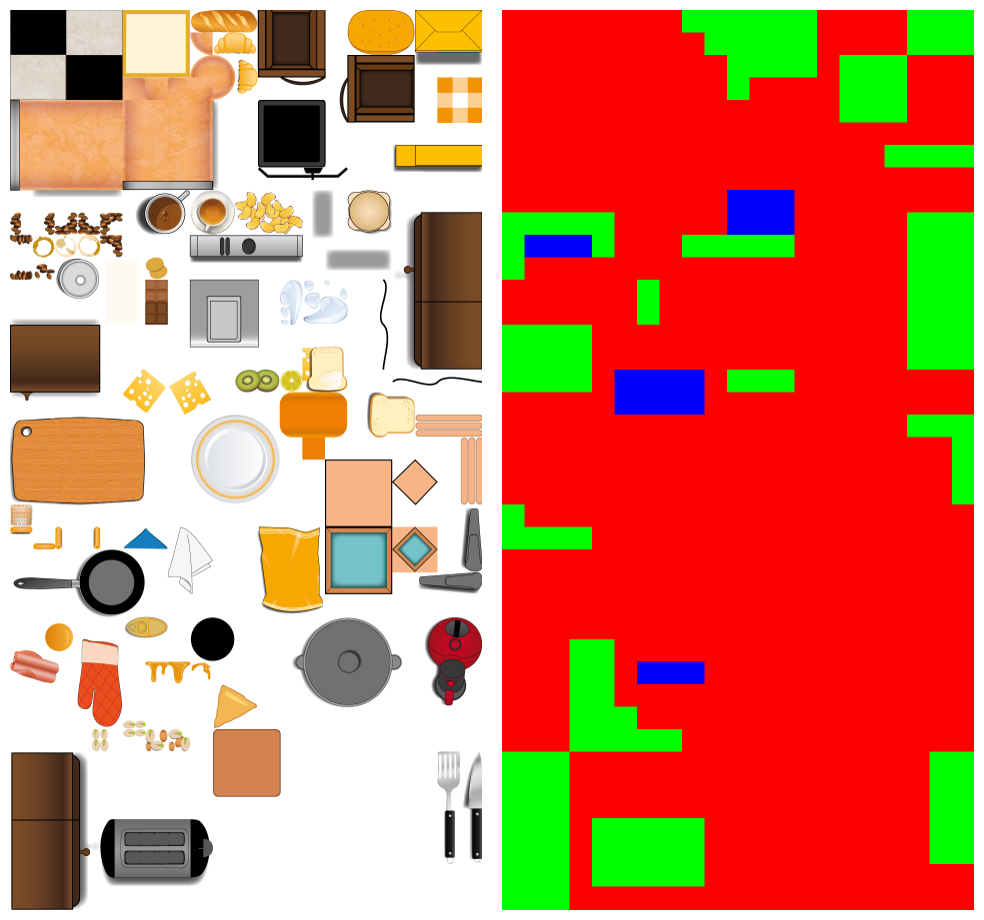
\includegraphics[scale=0.15]{imagenes/tileset-collisionmap.png}
        \end{center}
        

\end{frame}

\begin{frame}
    \frametitle{Colisiones}
    
    Una de las cosas más básicas en cualquier tipo de juego.

    \begin{block}{Colisión con el escenario}
        \begin{itemize}
            \item Detectamos si atravesamos algún tile no atravesable
            \item Si es así corregimos la posición del coche en según la dirección, sentido y lado del tile por
            el que colisione
            \item En el caso de que el tile sea de tipo realentizador, diminuimos la velocidad del coche
        \end{itemize}
    \end{block}

    \begin{center}
        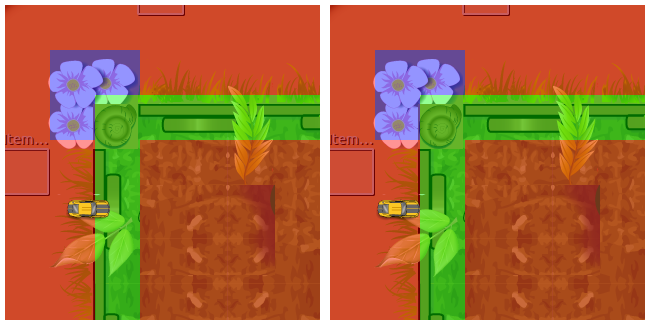
\includegraphics[scale=0.3]{imagenes/colision1-colision2.png}
    \end{center}
\end{frame}

\begin{frame}
    \frametitle{Colisiones}
    
    \begin{block}{Colisión entre vehículos}
        \begin{itemize}
            \item De forma similar a la colisión con el escenario
            \item Cuando se detecta la colisión se corrige la posición de los vehículos, en función la dirección, 
            sentido y lado del tile por el que colisionen
        \end{itemize}
    \end{block}
    
    \begin{block}{Colisión entre vehículos e ítems}
        \begin{itemize}
            \item Si es un ítem de ataque a distancia, destruiremos dicho ítem y cambiaremos el estado del coche con el que
            colisione
            \item Si el ítem es un obstaculo, cambiaremos el estado del coche en función del tipo de ítem
        \end{itemize}
    \end{block}

\end{frame}

\begin{frame}
    \frametitle{Inteligencia artificial}
    Otro de los aspectos más importante de un videojuego de las características de Zycars, es la
    inteligencia artificial, ya que en dos de los tres modos de juegos disponibles el objetivo es obtener la
    mejor clasificación posible, por delante de los demás coches controlados por el ordenador

        \begin{block}{Habilidades}
            \begin{itemize}
                \item Realización del recorrido: debe ser capaz de realizar los 
                recorridos de los circuitos.
                \item Lanzamiento de ítems: también debe poder usar los ítems que reciba de las bolas de ítems.
            \end{itemize}
        \end{block}
\end{frame}

\begin{frame}
    \frametitle{Realización del recorrido. Algoritmo A*}

    Aprovechando que tenemos un circuito creado por tiles y que podemos saber en todo momento en el tile 
    actual que se puede encontrar cualquiera de los competidores, se decidió implementar el 
    algoritmo de búsqueda A*.

        \begin{block}{Objetivo}
        Buscar el camino más corto y óptimo, en el caso de que exista, desde
        un nodo origen, hasta un nodo destino. A la hora de buscar dicho camino se tienen en cuenta factores
        como, el valor heurístico que poseen cada uno de los nodos, así como el coste real del recorrido.
        \end{block}

        \begin{block}{Parámetros}
        Los parametros que se tienen en cuenta en cada uno de los nodos.
            \begin{itemize}
                \item h’(n) es el valor heurístico del nodo actual n, hasta el final
                \item g(n) el coste real del camino desde el origen al nodo actual
                \item Función de evaluación: f(n) = g(n) + h’(n)
            \end{itemize}
        \end{block}

\end{frame}

\begin{frame}
    \frametitle{Realización del recorrido. Algoritmo A*}

        \begin{block}{Estructuras diferenciadas}
            \begin{itemize}
                \item Lista de abiertos: nodos por los que aún no se han pasado
                \item Lista de cerrados: nodos por los que ya se han pasado
            \end{itemize}
        \end{block}

        \begin{block}{Funcionamiento}
            Partiendo de un nodo en el que nos encontramos actualmente:
            \begin{enumerate}
                \item Obtenemos vecinos
                \item Comprobamos que no esten en abiertos ni cerrados
                \item Si alguno esta en abiertos, comprobamos su f(n), si es menor lo sustituiremos
                \item Introducimos en abiertos los que cumplan las condiciones
                \item Obtener de abiertos el nodo que tenga un f(n) menor y comenzamos de nuevo todo el proceso.
                \item Una vez lleguemos al nodo objetivo, detenemos la búsqueda y devolvemos el camino completo.
            \end{enumerate}
        \end{block}

\end{frame}

\begin{frame}
    \frametitle{Realización del recorrido. Algoritmo A*}

        Aplicación en Zycars

        \begin{center}
                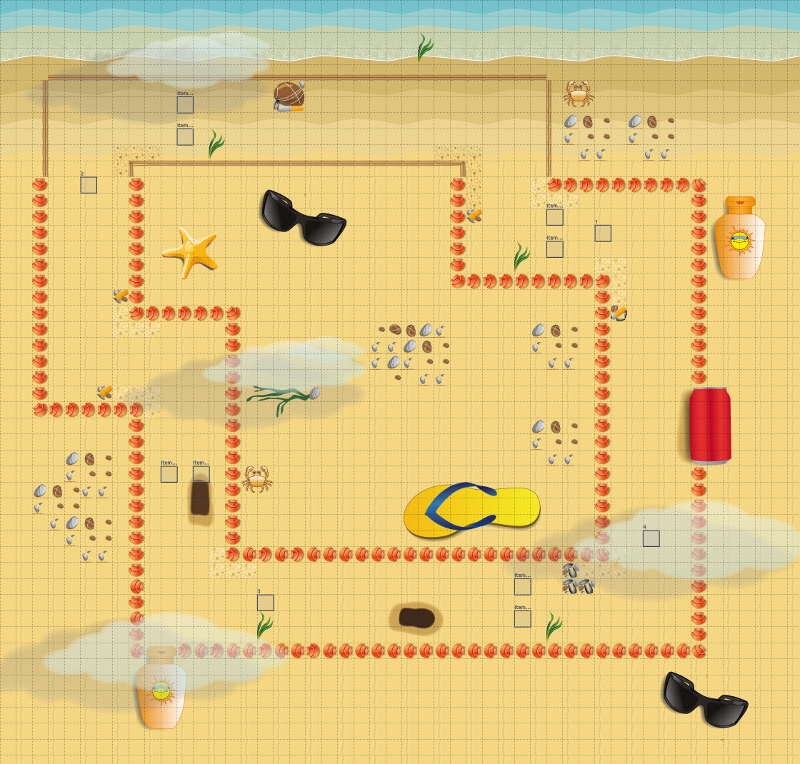
\includegraphics[scale=0.3]{imagenes/ia_check.png}
        \end{center}
        
\end{frame}

\begin{frame}
    \frametitle{Lanzamientos de ítems}

    Capaz de lanzar los ítems disponibles a los largo del juego, según las
    distintas situaciones en la que se encuentre.

        \begin{block}{Solución}
        Se eligió una forma muy sencilla y eficiente a la hora de realizarlo. Para ello cada
        vehículo controlado por la inteligencia artificial, tiene tanto un segmento que va desde el centro del
        coche hacia unos píxeles por delante de la posición actual del vehículo, como otro segmento que
        también va desde el centro pero uno píxeles atrás de la posición del vehículo.
        \end{block}

        \begin{center}
                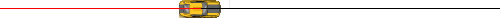
\includegraphics[scale=0.5]{imagenes/ia_segmentos.png}
        \end{center}

\end{frame}
